\documentclass{standalone}
\usepackage{mintikz}

\pgfdeclarelayer{background}
\pgfdeclarelayer{foreground}
\pgfsetlayers{background,main,foreground}
\usepackage{pifont}% http://ctan.org/pkg/pifont
\newcommand{\cmark}{\ding{51}}%
\newcommand{\xmark}{\ding{55}}%

\begin{document}
\thispagestyle{empty}
\begin{tikzpicture}[]
    %\draw[thin, black!20] (0,0) grid (20,-20);
    \tikzset{header/.style={draw, rounded corners, fill=#1!30},
    header/.default={gray}}
    % Start left
    \begin{scope}[local bounding box=TIRAGEBOX, yshift=0cm]
        %%%%%%%%%%%%%%%%%%%%%%%%%%%%%%%%%%%%%%%%%%%%%%%%%%%%%%%%%%%%%%%%%%%%%%%
        % Start TIRAGE
        \node[header=orchid, minimum width=5cm] (TIRAGEHEAD) at (0,0) {TIRAGE};
        %%%%%%%%%%%%%%%%%%%%%%%%%%%%%%%%%%%%%%%%%%%%%%%%%%%%%%%%%%%%%%%%%%%%%%%
        % WGTMAP
        \pgfplotstableread{../data/SDSS.txt}{\wgttable}
        \node[header=black, below=20pt]
            (WEIGTHMAP) at (TIRAGEHEAD.south) {WEIGTHMAP};
        \begin{axis}[name=Mwgt, scale=0.7,
            shift={($(WEIGTHMAP.south)+(0,-8pt)$)}, anchor=north,
            xmin=8, xmax=12.3,
            ymin=0, ymax=1,
            xlabel=$M_{\rm host}$, ylabel=$P(M)$,
            axis lines=left,
            clip=true]
            \addplot[black, samples=500]
                table[x=M, y=WGT] from \wgttable;
        \end{axis}
        %%%%%%%%%%%%%%%%%%%%%%%%%%%%%%%%%%%%%%%%%%%%%%%%%%%%%%%%%%%%%%%%%%%%%%%
        % Add space
        \node[minimum width=7cm] (SPACE) at (Mwgt.south) {} ;
        %%%%%%%%%%%%%%%%%%%%%%%%%%%%%%%%%%%%%%%%%%%%%%%%%%%%%%%%%%%%%%%%%%%%%%%
        % z DIST Rate from equation 6 of DES 2019
        % https://arxiv.org/pdf/1811.02379.pdf
        \begin{axis}[name=zdist, scale=0.7,
            at={(Mwgt.below south west)}, yshift=-1cm, anchor=north west,
            xmin=0, xmax=1.2,
            ymin=0, ymax=7.5,
            xlabel=$\bar{z}$, ylabel=\# (1$^{-15}$),
            axis lines=left,
            clip=true]
            \addplot[smooth, black]
                {1.75*(1+x)^2.11};
        \end{axis}
        %%%%%%%%%%%%%%%%%%%%%%%%%%%%%%%%%%%%%%%%%%%%%%%%%%%%%%%%%%%%%%%%%%%%%%%
        % START HOSTLIB
        % \matrix[matrix of nodes, anchor=west,
        %     row sep=-1pt, column sep=-\pgflinewidth,
        %     text width=40pt, align=center,
        %     %left delimiter=|,
        %     nodes={anchor=center, align=center}]
        %     (Mhostlib) at ([shift={(1, -1)}]Mwgt.south east)
        %     {$z$ & $M_{\rm host}$ & $x_1$ & $c$ \\
        %     \vdots & \vdots & \vdots & \vdots \\
        %     \vdots & \vdots & \vdots & \vdots \\
        %     \vdots & \vdots & \vdots & \vdots \\
        %     \vdots & \vdots & \vdots & \vdots \\
        %     \vdots & \vdots & \vdots & \vdots \\
        %     \vdots & \vdots & \vdots & \vdots \\
        %     \vdots & \vdots & \vdots & \vdots \\
        %     \vdots & \vdots & \vdots & \vdots \\
        %     \vdots & \vdots & \vdots & \vdots \\};
        % % Vlines
        % \foreach \n in {1, 2, 3}{
        % \draw[]
        %     (Mhostlib-1-\n.north east-|Mhostlib-10-\n.south east) |-
        % (Mhostlib-10-\n.south east);}
        % \draw[red, thick]
        %     ([shift={(0,-6pt)}]Mhostlib-5-1.north west) node [] (topleft) {}--
        %     (Mhostlib-5-1.south west) node [] (bottomleft) {} --
        %     (Mhostlib-5-4.south east) --
        %     ([shift={(0,-6pt)}]Mhostlib-5-4.north east) --
        %     cycle ;
        % % Wgt and Z to HOSTLIB
        % \draw[->]
        %     (Mwgt.east) -- (topleft);
        % \draw[->]
        %     (zdist.east) -- (bottomleft);
        % % HEADER
        % \node[header=black, above]
        %     (HOSTLIB) at (Mhostlib.north) {HOSTLIB};
    \end{scope}
    %%%%%%%%%%%%%%%%%%%%%%%%%%%%%%%%%%%%%%%%%%%%%%%%%%%%%%%%%%%%%%%%%%%%%%%%%%%
    \begin{scope}[local bounding box=SIMBOX, anchor=north west,
        shift={($(TIRAGEBOX.north east)+(2cm,0)$)}]
        %%%%%%%%%%%%%%%%%%%%%%%%%%%%%%%%%%%%%%%%%%%%%%%%%%%%%%%%%%%%%%%%%%%%%%%
        % Start TRUE
        \node[header=cornflowerblue, minimum width=10cm]
            (SIMHEAD) at (3,0) {SIMULATION};
        % Start timeseries
        % \node[anchor=north east] (TS) at ([shift={(-7cm,-0.5cm)}]SIMHEAD.south)
        \node[anchor=north east] (TS) at
            ([shift={(1cm,-1cm)}]SIMBOX.north west)
            {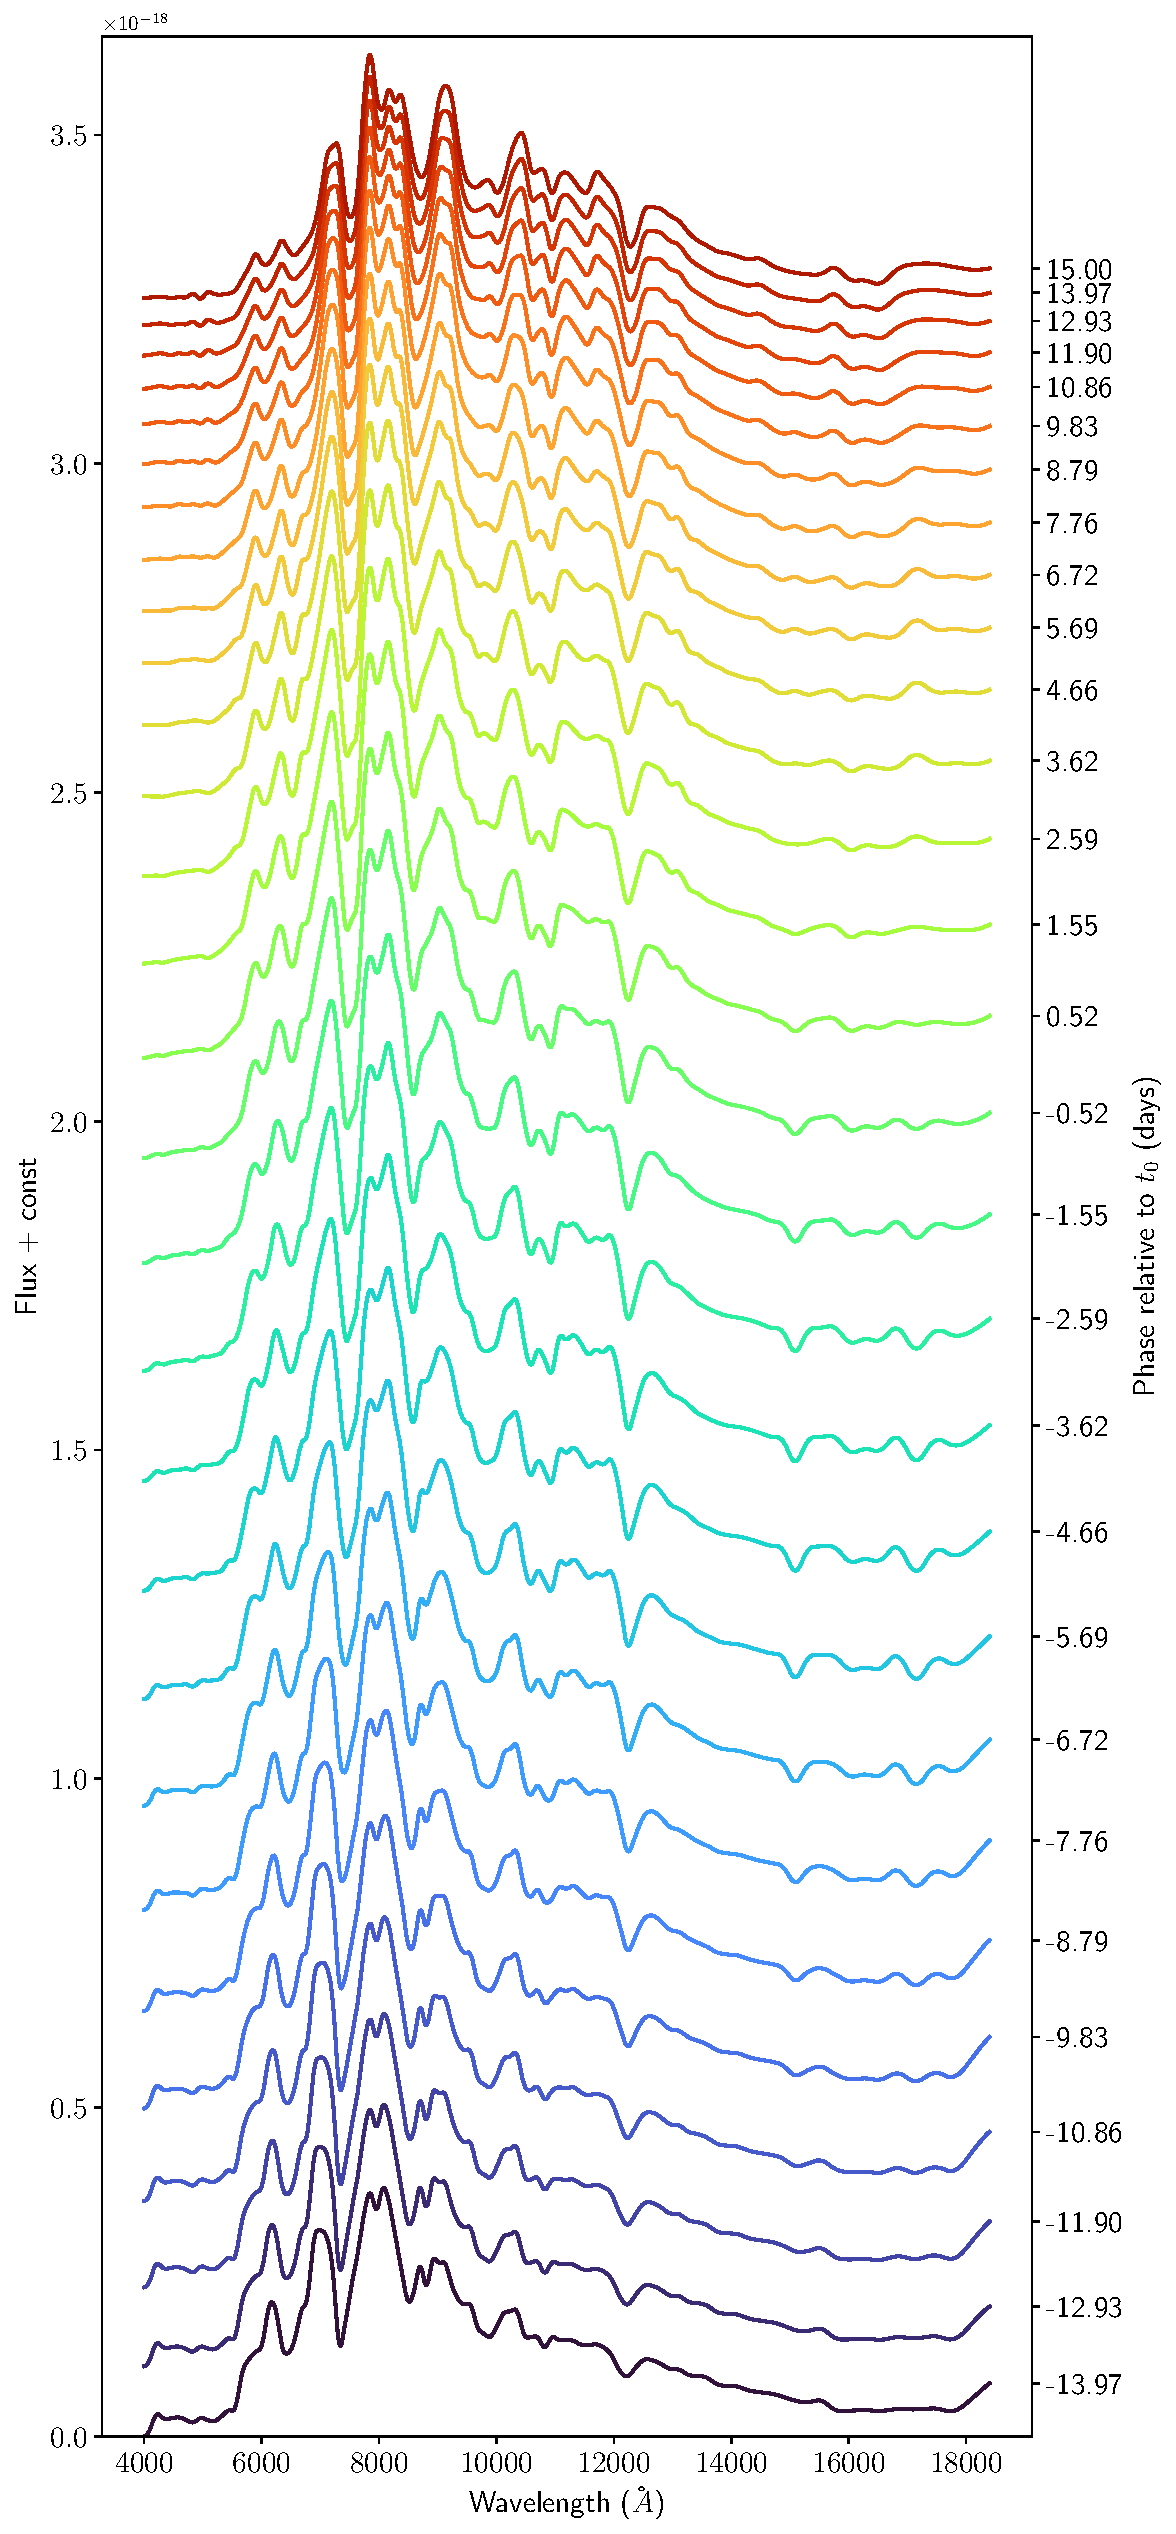
\includegraphics[scale=0.25]{timeseries.pdf}};
        \node[anchor=west, right, thick, scale=3] (plus) at
        (TS.east) {$\oplus$};
        %%%%%%%%%%%%%%%%%%%%%%%%%%%%%%%%%%%%%%%%%%%%%%%%%%%%%%%%%%%%%%%%%%%%%%%
        % SIMBLIB
        \matrix[matrix of nodes, anchor=west,
            row sep=-1pt, column sep=-\pgflinewidth,
            text width=40pt, align=center,
            %left delimiter=|,
            nodes={anchor=center, align=center}]
            (Msimlib) at (plus.east)
            {MJD & RADEC & Depth & Filter & PSF & $\cdots$ \\
            \vdots & \vdots & \vdots & \vdots & \vdots & \vdots\\
            \vdots & \vdots & \vdots & \vdots & \vdots & \vdots\\
            \vdots & \vdots & \vdots & \vdots & \vdots & \vdots\\
            \vdots & \vdots & \vdots & \vdots & \vdots & \vdots\\
            \vdots & \vdots & \vdots & \vdots & \vdots & \vdots\\};
        % Vlines
        \foreach \n in {1, 2, 3, 4, 5}{
        \draw[]
            (Msimlib-1-\n.north east-|Msimlib-6-\n.south east) |-
        (Msimlib-6-\n.south east);}
        % HOSTLIB z to hostmass
        % \draw[->]
        %     ([shift={(-10pt,0)}]Mhostlib-1-2.east) --
        %     ([shift={(+10pt,0)}]Mhostlib-1-3.west);
        % HEADER
        \node[header=black, above]
            (SIMLIB) at (Msimlib.north) {SIMLIB};
        %%%%%%%%%%%%%%%%%%%%%%%%%%%%%%%%%%%%%%%%%%%%%%%%%%%%%%%%%%%%%%%%%%%%%%%
        % Bands and LC
        \node[anchor=north] (TSDSS) at ([shift={(2cm,0cm)}]TS.south)
            {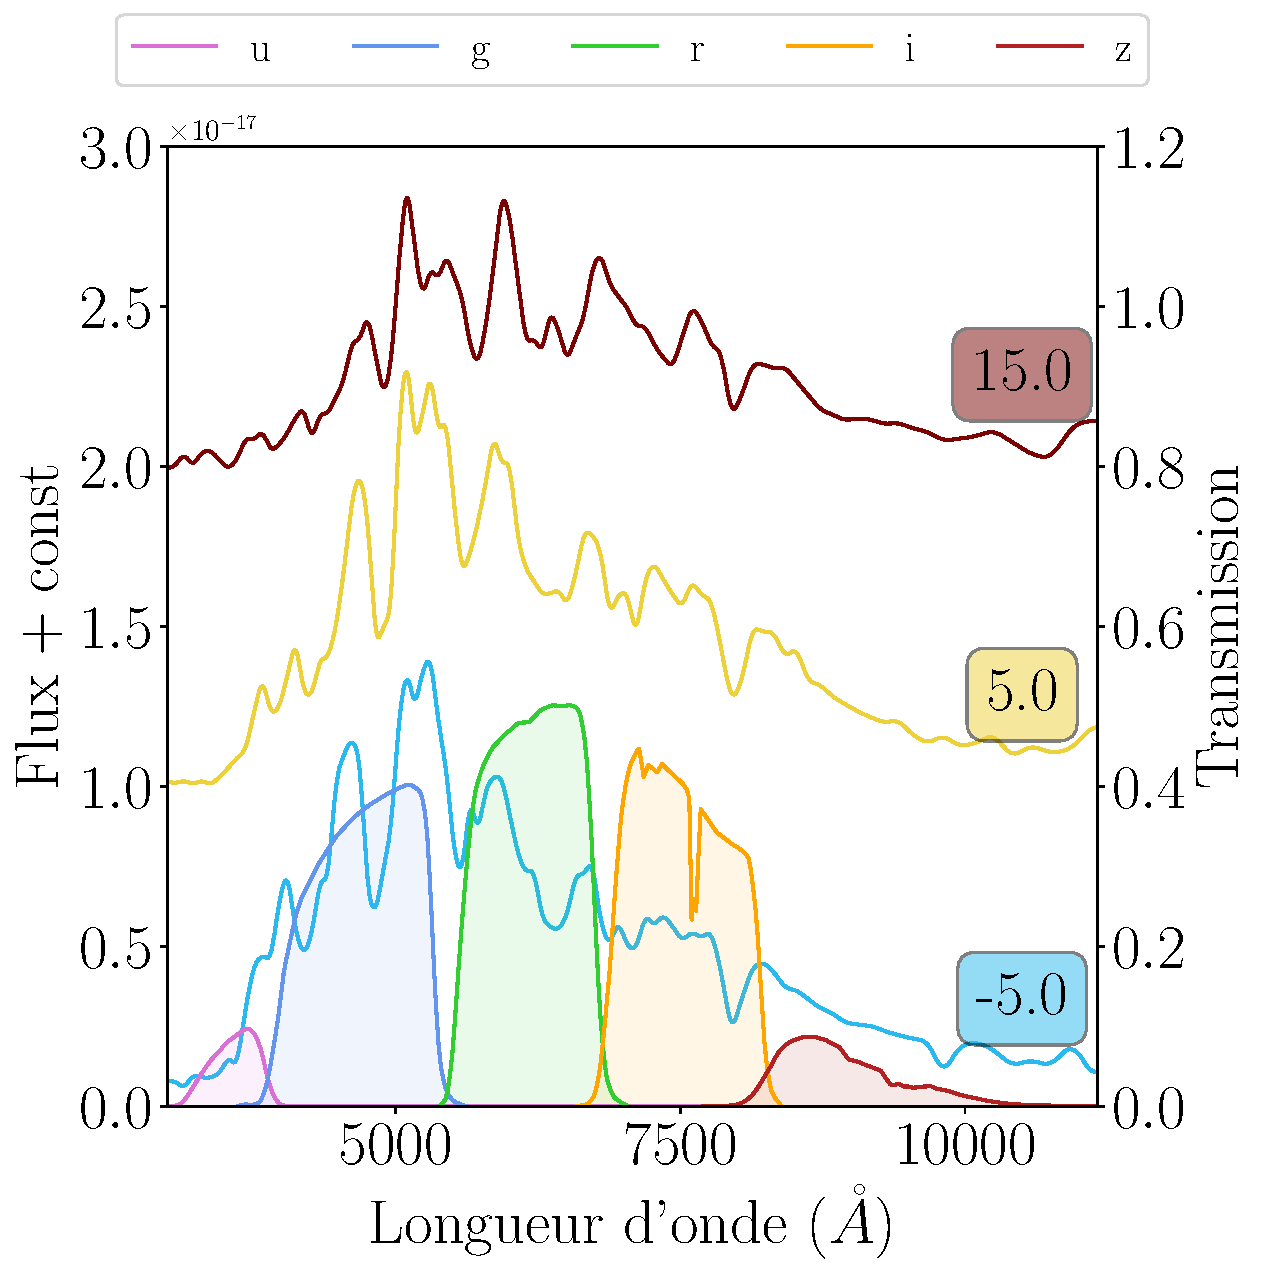
\includegraphics[width=5cm]{timeseries_sdss.pdf}};
        \node[anchor=west] (SDLC) at ([shift={(3cm,0)}]TSDSS.east)
            {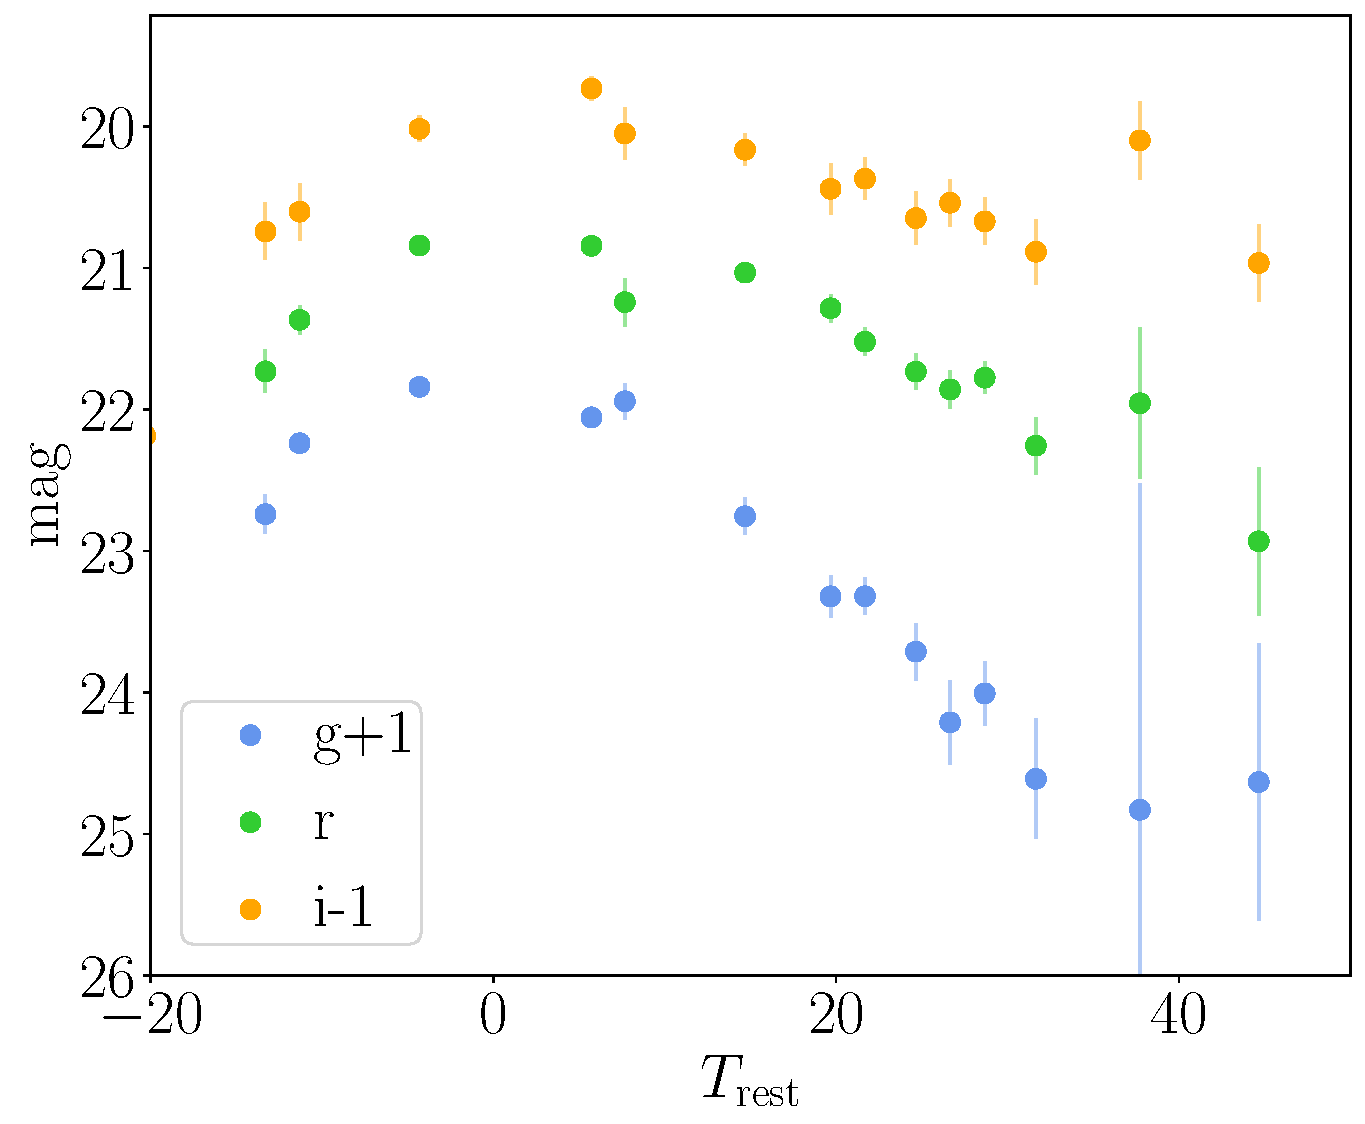
\includegraphics[width=6cm]{lc_2005gg_NOSALT.pdf}};
        %%%%%%%%%%%%%%%%%%%%%%%%%%%%%%%%%%%%%%%%%%%%%%%%%%%%%%%%%%%%%%%%%%%%%%%
        \draw[rounded corners]
            (TS.north west) --
            (TS.south west) node [right] (corner) {} --
            (TS.south east -| Msimlib.south east) --
            (Msimlib.north east |- TS.north east) -- cycle;
        %%%%%%%%%%%%%%%%%%%%%%%%%%%%%%%%%%%%%%%%%%%%%%%%%%%%%%%%%%%%%%%%%%%%%%%
        % Arrows
            \draw[thick, ->] ([shift={(1cm,0)}]corner.south west) |- (TSDSS.west) ;
        \draw[->] (TSDSS.east) -- (SDLC.west);
    \end{scope}
    %%%%%%%%%%%%%%%%%%%%%%%%%%%%%%%%%%%%%%%%%%%%%%%%%%%%%%%%%%%%%%%%%%%%%%%
    \begin{pgfonlayer}{background}
        \draw[fill=orchid!10, rounded corners]
        ([shift={(0, -2pt)}]TIRAGEBOX.north east |- TIRAGEHEAD.south east) --
        ([shift={(0, -2pt)}]TIRAGEBOX.north west |- TIRAGEHEAD.south west) --
        (TIRAGEBOX.south west) --
        (TIRAGEBOX.south east) --
        cycle ;
            % (PRIORBOX.north east |- TRUEBOX.north west) --
            % (PRIORBOX.north west |- TRUEBOX.north west) --
            % (PRIORBOX.north west |- TRUEBOX.south west) --
            % (TRUEBOX.south west -| PRIORBOX.south east) -- cycle ;
    \end{pgfonlayer}
    \begin{pgfonlayer}{background}
        \draw[fill=cornflowerblue!10, rounded corners]
        ([shift={(0, -2pt)}]SIMBOX.north east |- SIMHEAD.south east) --
        ([shift={(0, -2pt)}]SIMBOX.north west |- SIMHEAD.south west) --
        (SIMBOX.south west) --
        (SIMBOX.south east) --
        cycle ;
            % (PRIORBOX.north east |- TRUEBOX.north west) --
            % (PRIORBOX.north west |- TRUEBOX.north west) --
            % (PRIORBOX.north west |- TRUEBOX.south west) --
            % (TRUEBOX.south west -| PRIORBOX.south east) -- cycle ;
    \end{pgfonlayer}
    %%%%%%%%%%%%%%%%%%%%%%%%%%%%%%%%%%%%%%%%%%%%%%%%%%%%%%%%%%%%%%%%%%%%%%%
    % \begin{scope}[local bounding box=SURVEYBOX,
    %     shift={($(TRUE.east)+(9cm,0)$)}]
    %     \node[header=cornflowerblue] (SURVEY) at (0,0) {SONDAGE};
    %     \node[] (TSDSS) at ([shift={(0,-5)}]SURVEY.center)
    %         {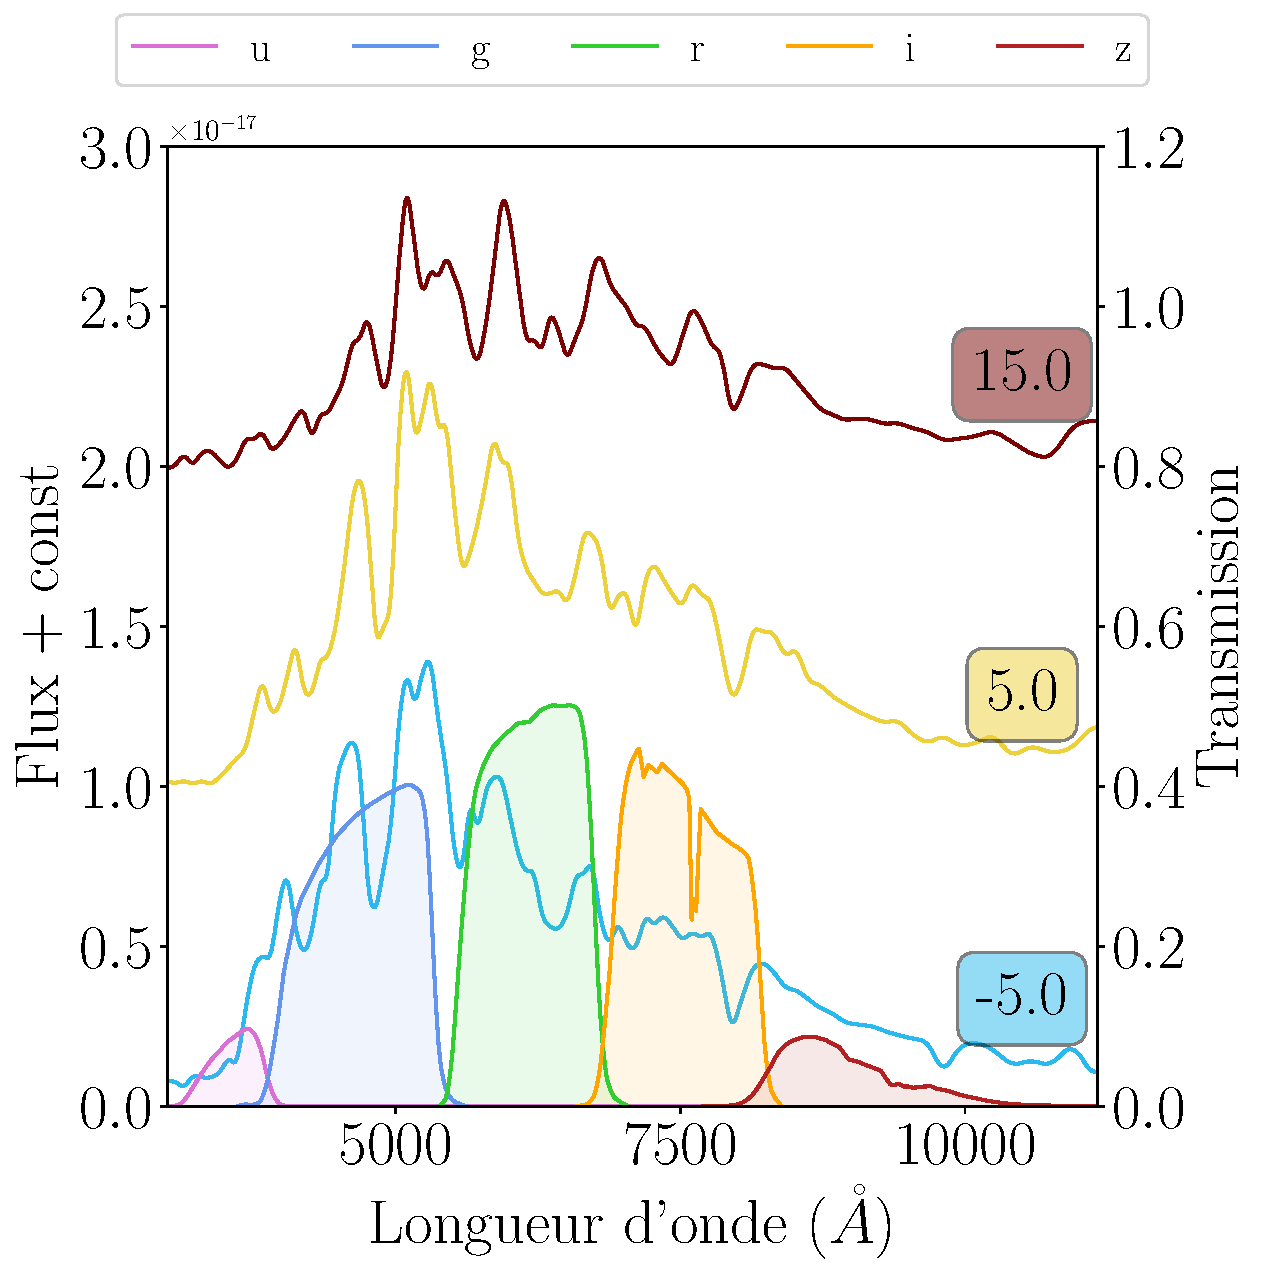
\includegraphics[scale=0.3]{timeseries_sdss.pdf}};
    %     \node[] (SDLC) at ([shift={(0,-5)}]TSDSS.south)
    %         {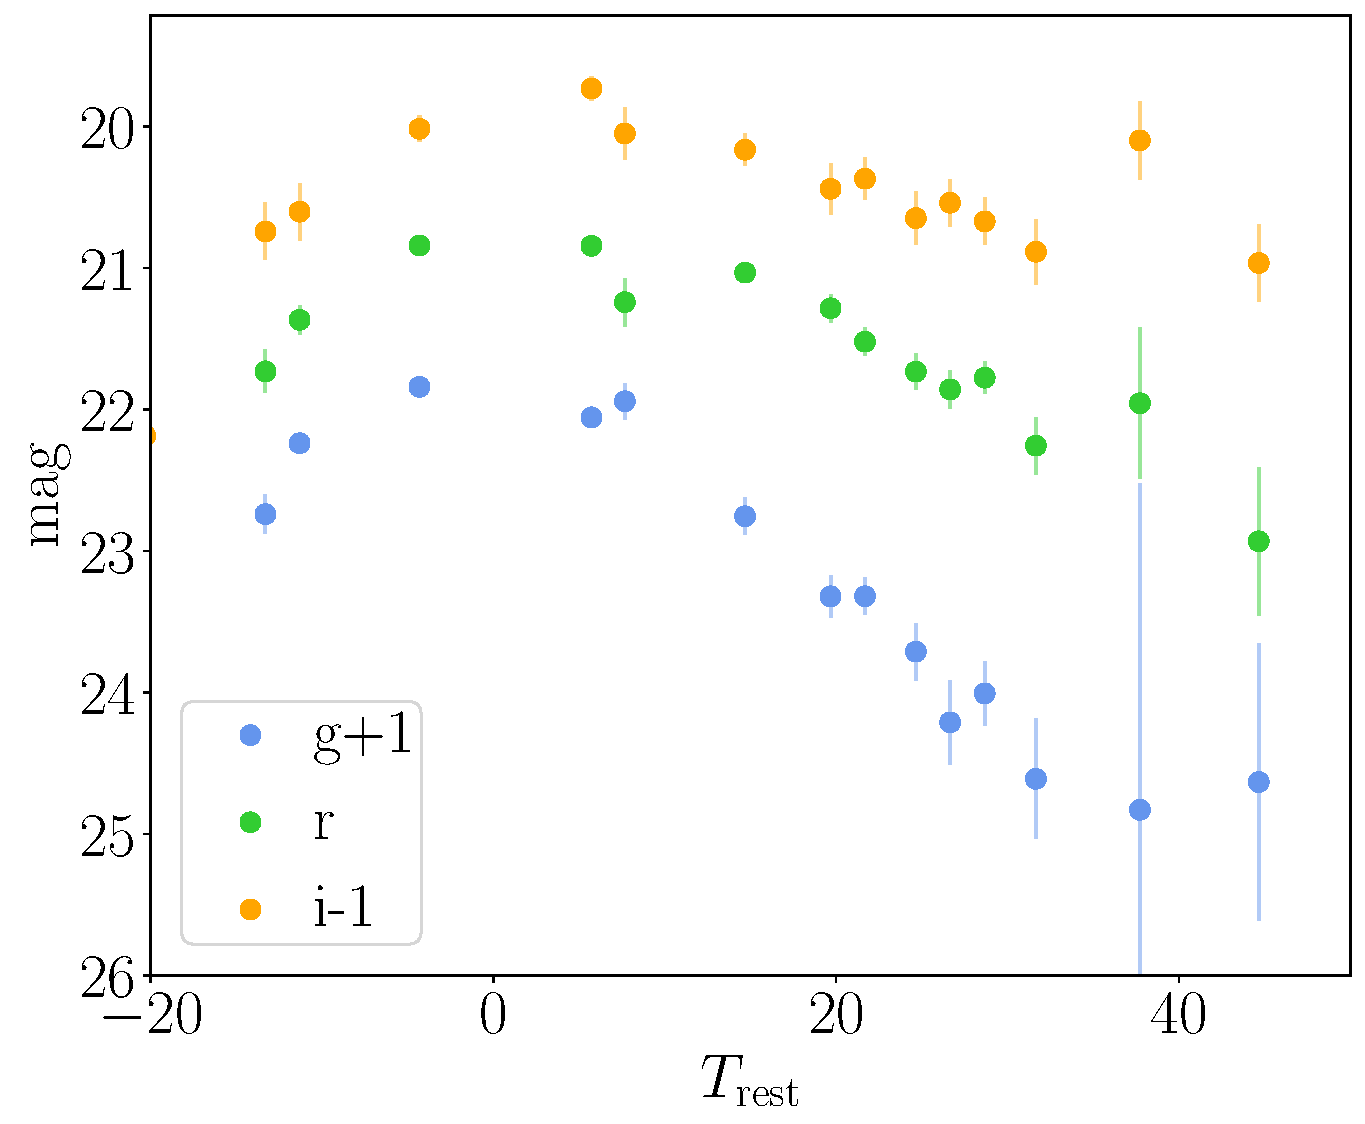
\includegraphics[scale=.5]{lc_2005gg_NOSALT.pdf}};
    %     \draw[->] (TSDSS.south) -- (SDLC.north);
    % \end{scope}
    % %%%%%%%%%%%%%%%%%%%%%%%%%%%%%%%%%%%%%%%%%%%%%%%%%%%%%%%%%%%%%%%%%%%%%%%
    % \begin{pgfonlayer}{background}
    %     \draw[fill=cornflowerblue!20, rounded corners]
    %         (SURVEYBOX.north east) -- (SURVEYBOX.north west) --
    %         (SURVEYBOX.north west |- TRUEBOX.south west) --
    %         (TRUEBOX.south east -| SURVEYBOX.south east) -- cycle ;
    % \end{pgfonlayer}
    % %%%%%%%%%%%%%%%%%%%%%%%%%%%%%%%%%%%%%%%%%%%%%%%%%%%%%%%%%%%%%%%%%%%%%%%
    % \begin{scope}[local bounding box=SELECTIONBOX,
    %     shift={($(SURVEY.east)+(7.9cm,0)$)}]
    %     % Start SELECTION
    %     \node[header=limegreen] (SELECTION) at (0,0) {S\'ELECTION};
    %     % Start PHOTSEL
    %     \node[header=limegreen]
    %         (PHOTSEL) at ([shift={(0,-2)}]SELECTION.center) {Photom\'etrique};
    %     \matrix[matrix of nodes, anchor=north,
    %         row sep=-1pt, column sep=-\pgflinewidth,
    %         text width=60pt, align=center,
    %         %left delimiter=|,
    %         nodes={anchor=center, align=center}]
    %         (PHOTLIST) at ([shift={(0,-0.2cm)}]PHOTSEL.south)
    %         {$T_{\rm rest} < 0$ & $T_{\rm rest} > 10$ & SNR > 5 $gri$ & $\cdots$ \\
    %         \cmark & \cmark & \xmark \\
    %         \cmark & \cmark & \xmark \\
    %         \xmark & \xmark & \cmark \\
    %         \xmark & \cmark & \xmark \\
    %         \vdots & \vdots & \vdots \\};
    %     % Vlines
    %     \foreach \n in {1, 2, 3}{
    %     \draw[]
    %         (PHOTLIST-1-\n.north east-|PHOTLIST-6-\n.south east) |-
    %     (PHOTLIST-6-\n.south east);}
    %     % Start SPECSEL
    %     \node[header=limegreen]
    %         (SPECSEL) at ([shift={(0,-2)}]PHOTLIST.south) {Spectroscopique};
    %     %%%%%%%%%%%%%%%%%%%%%%%%%%%%%%%%%%%%%%%%%%%%%%%%%%%%%%%%%%%%%%%%%%%%%%%
    %     % SDSS SPECEFF from sdss spec
    %     \pgfplotstableread{../data/sdss_spec.dat}{\sdspectable}
    %     \findMax{\sdspectable}{r}{\rmax}
    %     \begin{axis}[name=sdspec, scale=0.8,
    %         at={(SPECSEL.south west)}, anchor=north west,
    %         yshift=-1cm, xshift=-1cm,
    %         xmin=16.0, xmax=\rmax*0.8,
    %         ymin=0, ymax=1.0,
    %         xlabel=$r$ (mag), ylabel=\'Efficacit\'e spectroscopique,
    %         axis lines=left,
    %         clip=true]
    %         \addplot[black, smooth]
    %             table[x=r, y=SPECEFF] from \sdspectable;
    %     \end{axis}
    %     % \matrix[matrix of nodes, anchor=north,
    %     %     row sep=-1pt, column sep=-\pgflinewidth,
    %     %     text width=40pt, align=center,
    %     %     %left delimiter=|,
    %     %     nodes={anchor=center, align=center}]
    %     %     (SPECLIST) at ([shift={(0,-0.2cm)}]SPECSEL.south)
    %     %     {$z$ | & Date | & RADEC \\
    %     %     \vdots & \vdots & \vdots \\};
    % \end{scope}
    % %%%%%%%%%%%%%%%%%%%%%%%%%%%%%%%%%%%%%%%%%%%%%%%%%%%%%%%%%%%%%%%%%%%%%%%
    % \begin{pgfonlayer}{background}
    %     \draw[fill=limegreen!20, rounded corners]
    %         (SELECTIONBOX.north east) -- (SELECTIONBOX.north west) --
    %         (SELECTIONBOX.north west |- TRUEBOX.south west) --
    %         (TRUEBOX.south east -| SELECTIONBOX.south east) -- cycle ;
    % \end{pgfonlayer}
    % %%%%%%%%%%%%%%%%%%%%%%%%%%%%%%%%%%%%%%%%%%%%%%%%%%%%%%%%%%%%%%%%%%%%%%%
    % \begin{scope}[local bounding box=CONSBOX,
    %     shift={($(SELECTION.east)+(5cm,0)$)}]
    % %%%%%%%%%%%%%%%%%%%%%%%%%%%%%%%%%%%%%%%%%%%%%%%%%%%%%%%%%%%%%%%%%%%%%%%
    %     % Start CONS
    %     \node[header=orange] (CONS) at (3,0) {CONSERV\'E};
    %     %%%%%%%%%%%%%%%%%%%%%%%%%%%%%%%%%%%%%%%%%%%%%%%%%%%%%%%%%%%%%%%%%%%%%%%
    %     % M DIST from dumps and 2_LCFIT
    %     \pgfplotstableread{../data/mTrue_SDSS.txt}{\mtrue}
    %     \pgfplotstableread{../data/mSelected_SDSS.txt}{\msel}
    %     \pgfplotstableread{../data/mFitted_SDSS.txt}{\mfit}
    %     \begin{axis}[name=mdump, scale=0.7,
    %         yshift=-1.5cm, anchor=north west,
    %         xmin=7, xmax=12.1,
    %         ymin=0, ymax=0.73,
    %         xlabel=$M$, ylabel=$P$,
    %         axis lines=left,
    %         legend pos=north west,
    %         clip=false]
    %         \addplot[smooth, orchid, line width=2pt]
    %             table[x=mlin, y=values] from \mtrue;
    %         \addlegendentry{V\'erit\'e}
    %         \addplot[smooth, limegreen, line width=2pt]
    %             table[x=mlin, y=values] from \msel;
    %         \addlegendentry{S\'electionn\'e}
    %         \addplot[smooth, orange, line width=2pt]
    %             table[x=mlin, y=values] from \mfit;
    %         \addlegendentry{Ajust\'e}
    %     \end{axis}
    %     %%%%%%%%%%%%%%%%%%%%%%%%%%%%%%%%%%%%%%%%%%%%%%%%%%%%%%%%%%%%%%%%%%%%%%%
    %     % X1 DIST dumps and 2_LCFIT
    %     \pgfplotstableread{../data/xTrue_SDSS.txt}{\xtrue}
    %     \pgfplotstableread{../data/xSelected_SDSS.txt}{\xsel}
    %     \pgfplotstableread{../data/xFitted_SDSS.txt}{\xfit}
    %     \begin{axis}[name=xdump, scale=0.7,
    %         at={(mdump.below south west)},
    %         yshift=-0.3cm, anchor=north west,
    %         xmin=-3, xmax=3,
    %         ymin=0, ymax=0.5,
    %         xlabel=$x_1$, ylabel=$P$,
    %         axis lines=left,
    %         legend pos=north west,
    %         clip=false]
    %         \addplot[smooth, orchid, line width=2pt]
    %             table[x=xlin, y=values] from \xtrue;
    %         % \addlegendentry{V\'erit\'e}
    %         \addplot[smooth, limegreen, line width=2pt]
    %             table[x=xlin, y=values] from \xsel;
    %         % \addlegendentry{S\'electionn\'e}
    %         \addplot[smooth, orange, line width=2pt]
    %             table[x=xlin, y=values] from \xfit;
    %         % \addlegendentry{Ajust\'e}
    %     \end{axis}
    %     %%%%%%%%%%%%%%%%%%%%%%%%%%%%%%%%%%%%%%%%%%%%%%%%%%%%%%%%%%%%%%%%%%%%%%%
    %     % C DIST dumps and 2_LCFIT
    %     \pgfplotstableread{../data/cTrue_SDSS.txt}{\ctrue}
    %     \pgfplotstableread{../data/cSelected_SDSS.txt}{\csel}
    %     \pgfplotstableread{../data/cFitted_SDSS.txt}{\cfit}
    %     \begin{axis}[name=cdump, scale=0.7,
    %         at={(xdump.below south west)},
    %         yshift=-0.3cm, anchor=north west,
    %         xmin=-0.3, xmax=0.4,
    %         ymin=0, ymax=7.2,
    %         xlabel=$c$, ylabel=$P$,
    %         axis lines=left,
    %         legend pos=north west,
    %         clip=false]
    %         \addplot[smooth, orchid, line width=2pt]
    %             table[x=clin, y=values] from \ctrue;
    %         % \addlegendentry{V\'erit\'e}
    %         \addplot[smooth, limegreen, line width=2pt]
    %             table[x=clin, y=values] from \csel;
    %         % \addlegendentry{S\'electionn\'e}
    %         \addplot[smooth, orange, line width=2pt]
    %             table[x=clin, y=values] from \cfit;
    %         % \addlegendentry{Ajust\'e}
    %     \end{axis}
    %     %%%%%%%%%%%%%%%%%%%%%%%%%%%%%%%%%%%%%%%%%%%%%%%%%%%%%%%%%%%%%%%%%%%%%%%
    %     % Z DIST dumps and 2_LCFIT
    %     \pgfplotstableread{../data/zTrue_SDSS.txt}{\ztrue}
    %     \findMax{\ztrue}{zlin}{\zxmax}
    %     \findMax{\ztrue}{values}{\zymax}
    %     \pgfplotstableread{../data/zSelected_SDSS.txt}{\zsel}
    %     \pgfplotstableread{../data/zFitted_SDSS.txt}{\zfit}
    %     \begin{axis}[name=zdump, scale=0.7,
    %         at={(cdump.below south west)},
    %         yshift=-0.3cm, anchor=north west,
    %         xmin=0, xmax=\zxmax,
    %         ymin=0, ymax=\zymax,
    %         xlabel=$z$, ylabel=$P$,
    %         axis lines=left,
    %         legend pos=north west,
    %         clip=false]
    %         \addplot[smooth, orchid, line width=2pt]
    %             table[x=zlin, y=values] from \ztrue;
    %         % \addlegendentry{V\'erit\'e}
    %         \addplot[smooth, limegreen, line width=2pt]
    %             table[x=zlin, y=values] from \zsel;
    %         % \addlegendentry{S\'electionn\'e}
    %         \addplot[smooth, orange, line width=2pt]
    %             table[x=zlin, y=values] from \zfit;
    %         % \addlegendentry{Ajust\'e}
    %     \end{axis}
    %     %%%%%%%%%%%%%%%%%%%%%%%%%%%%%%%%%%%%%%%%%%%%%%%%%%%%%%%%%%%%%%%%%%%%%%%
    % \end{scope}
    % %%%%%%%%%%%%%%%%%%%%%%%%%%%%%%%%%%%%%%%%%%%%%%%%%%%%%%%%%%%%%%%%%%%%%%%
    % \begin{pgfonlayer}{background}
    %     \draw[fill=orange!20, rounded corners]
    %         (CONSBOX.north east) -- (CONSBOX.north west) --
    %         (CONSBOX.north west |- TRUEBOX.south west) --
    %         (TRUEBOX.south east -| CONSBOX.south east) -- cycle ;
    % \end{pgfonlayer}
    % %%%%%%%%%%%%%%%%%%%%%%%%%%%%%%%%%%%%%%%%%%%%%%%%%%%%%%%%%%%%%%%%%%%%%%%
    % % \begin{scope}[shift={(16,0)}]
    % %     \node[header=red] (SIMRES) at (0,0) {Simulation propreties};
    % % \end{scope}
    % % \begin{scope}[shift={(20,0)}]
    % %     \node[header=blue] (LCFIT) at (0,0) {LC fit};
    % % \end{scope}
\end{tikzpicture}
\end{document}
